% Session 5 -- same gap, different topology: trivial s-wave versus chiral p-wave.
% Placement: sec. "Same gap, different topology", after the bulk-boundary paragraph.
% Rendered by figures/blender/s05f04_topology.py, labels in figures/overlays/s05f04_topology.tex.
\begin{aqmfigure}{fig:s05:topology}{Two gaps that a spectroscopy experiment cannot distinguish, seen
from above. Each dial is the phase of $\Delta(\mathbf k)$, an arrow in the complex plane, drawn at
the point of the Fermi pocket where it is evaluated. (a) For $s$-wave pairing this phase is the same
everywhere, so as $\mathbf k$ goes once around the pocket the value of $\Delta$ stays at a single
point of the complex plane, with winding number zero and Chern number zero. (b) For chiral $p$-wave
pairing (5.15) the phase instead follows the direction of $\mathbf k$, so $\Delta$ draws a loop that
encircles the origin once. The modulus is essentially the same in both cases, so both fully gap the
same pocket by the same amount. Only the winding is different, and the winding is what the Chern
number counts. (c) The consequence in a finite sample. The trivial state is gapped at its boundary
as well as in its bulk, while the chiral state must have $|C|$ gapless branches on each edge, all
going in the same direction, and in the opposite direction on the opposite edge. Here $C=\pm2$, with
one branch from each of the two identical spin blocks of (5.8).}
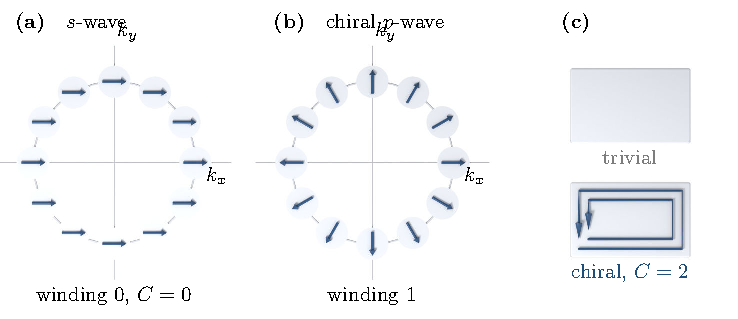
\includegraphics{figures/pdf/s05f04_topology.pdf}
\end{aqmfigure}
